% ! TeX root = ../../../master-thesis.tex

\subsection{FRASP}
\label{section:background:technologies:frasp}

\textbf{FRASP (Functional Reactive Approach to Self-organization Programming)}\footnote{Repository at: \url{https://github.com/cric96/distributed-frp}}
is a new open-source aggregate computing framework for the Scala programming
language, currently under active research.

FRASP draws inspiration from \ac{ScaFi}, sharing many similarities. The key
distinction lies in the implemented execution model: the former adopts a novel
functional reactive execution model, leveraging the Sodium library, as opposed
to the round-based execution model of the latter, common in aggregate computing
\cite{FRASP}.

The motivation behind FRASP is to provide for some of the shortcomings of the
round-based execution model, including \textit{periodic computation},
\textit{complete re-computation} and \textit{redundant message exchanges}.
Indeed, the benefits of adopting the execution model of FRASP for aggregate
computing are the following:
\begin{itemize}
  \item \textit{Event-driven computation}: in a device, computation is driven
        by relevant changes in its perception of the environment (e.g.,
        sensors, neighbour data). As a result, computation is performed
        only when required.
  \item \textit{Independent scheduling of sub-computations}: when a device
        detects a change in its context, only the dependent sub-computations
        of its programs are re-computed. In other words, complete
        re-computations of an aggregate specification are avoided when possible.
  \item \textit{Minimal communication}: a device only broadcasts its exports
        upon relevant changes, avoiding further message exchanges after the
        aggregate reaches a stable configuration. As a consequence, redundant
        computation caused by repeated messages is avoided.
\end{itemize}

In FRASP, computational fields are reified into Sodium's \texttt{Cell}s, which
neatly capture their time-varying nature. Like \ac{FRP}, a specification is the
configuration of a computational graph, which tracks the dependencies between
computational fields and manages the propagation of change automatically.

Computational fields are initialized by \texttt{Flow}s, which model
sub-computations in an aggregate specification and are first-class citizens in
FRASP. The purpose of \texttt{Flow}s is to defer the construction of the
computational graph until the devices of the aggregate network are initialized,
which is required to express dependencies related to their neighbours and
sensors. In addition, \texttt{Flow}s keep track of their position inside the
FRASP specification, building the abstract syntax tree used for alignment.

The semantics of FRASP (Listing \ref{listing:frasp-language}) faithfully
resembles the semantics of field calculus, while also sharing common constructs
with \ac{ScaFi}. However, since computational fields have been reified,
additional operators are required to adapt values yielded by plain Scala
expressions to the language constructs, namely \texttt{constant} for values and
\texttt{lift} for operators (\textit{lifting}).

The main difference with the field calculus semantics is the \texttt{loop}
construct, replacing the \texttt{rep} construct. The \texttt{loop} construct
implements the evolution of a computational field over time as a (cyclic)
self-dependency within the computational graph of a FRASP specification, rather
than relying on the concept of computation round. Indeed, the previous state of
a device is computed through self-alignment, leveraging the fact that every
device is a neighbour of itself.

\lstinputlisting[
  language=Scala,
  caption={The core constructs of the FRASP language, represented as a trait,
      abstracting over the actual organization within FRASP.},
  captionpos=b,
  label={listing:frasp-language}
]{resources/listings/frasp-language.txt}

FRASP also provides a basic simulator implementing its reactive execution model
(Figures \ref{figure:frasp-simulation} and
\ref{figure:frasp-simulation-example}). On an abstract level, the simulator
operates in two phases:
\begin{itemize}
  \item \textbf{Configuration}: accept a FRASP specification, which describes
        the structure of a computational graph, and an environment, which
        describes the devices of the aggregate and their neighbouring relations
        (e.g., based on proximity).
  \item \textbf{Execution}: create the devices, based on the environment, and
        build the computational graph of the aggregate, based on the FRASP
        specification. In doing so, the simulator establishes the dependency
        chains from the percepts of each device (i.e., neighbour and
        environmental data) to its exports and from its exports to the
        neighbour data perceived by its neighbours. As soon as the graph is
        built, the \textit{input nodes}\footnote{
          An input node is node initialized by a leaf \texttt{Flow} in the
          abstract syntax tree of a FRASP specification: either
          \texttt{constant}, \texttt{mid}, \texttt{sensor}, \texttt{nbrSensor}
          or \texttt{loop}, as they do not require other \texttt{Flow}s in
          input.
        } of the computational graph will propagate their initial value to all
        their dependents, then the computation is carried on automatically by
        the underlying \ac{FRP} engine indefinitely.

        Since non-trivial specifications for aggregate computing include cyclic
        dependencies in the computational graph, additional measures must be
        taken to avoid the indefinite propagation of non-relevant changes
        (e.g., redundant messages). In particular, FRASP applies the FRP
        calming pattern to all nodes when building a computational graph,
        allowing self-stabilising specifications to eventually reach a stable
        state, in which events are no longer propagated in the aggregate until
        the next change in the environment. Note that the execution may
        continue indefinitely even after reaching a stable state, since it is
        always possible for an event to happen in the future, however, no
        propagation of change implies no consumption of computational resources
        (i.e., the aggregate keeps waiting for an event to occur).
\end{itemize}

\begin{figure}[!ht]
  \centering
  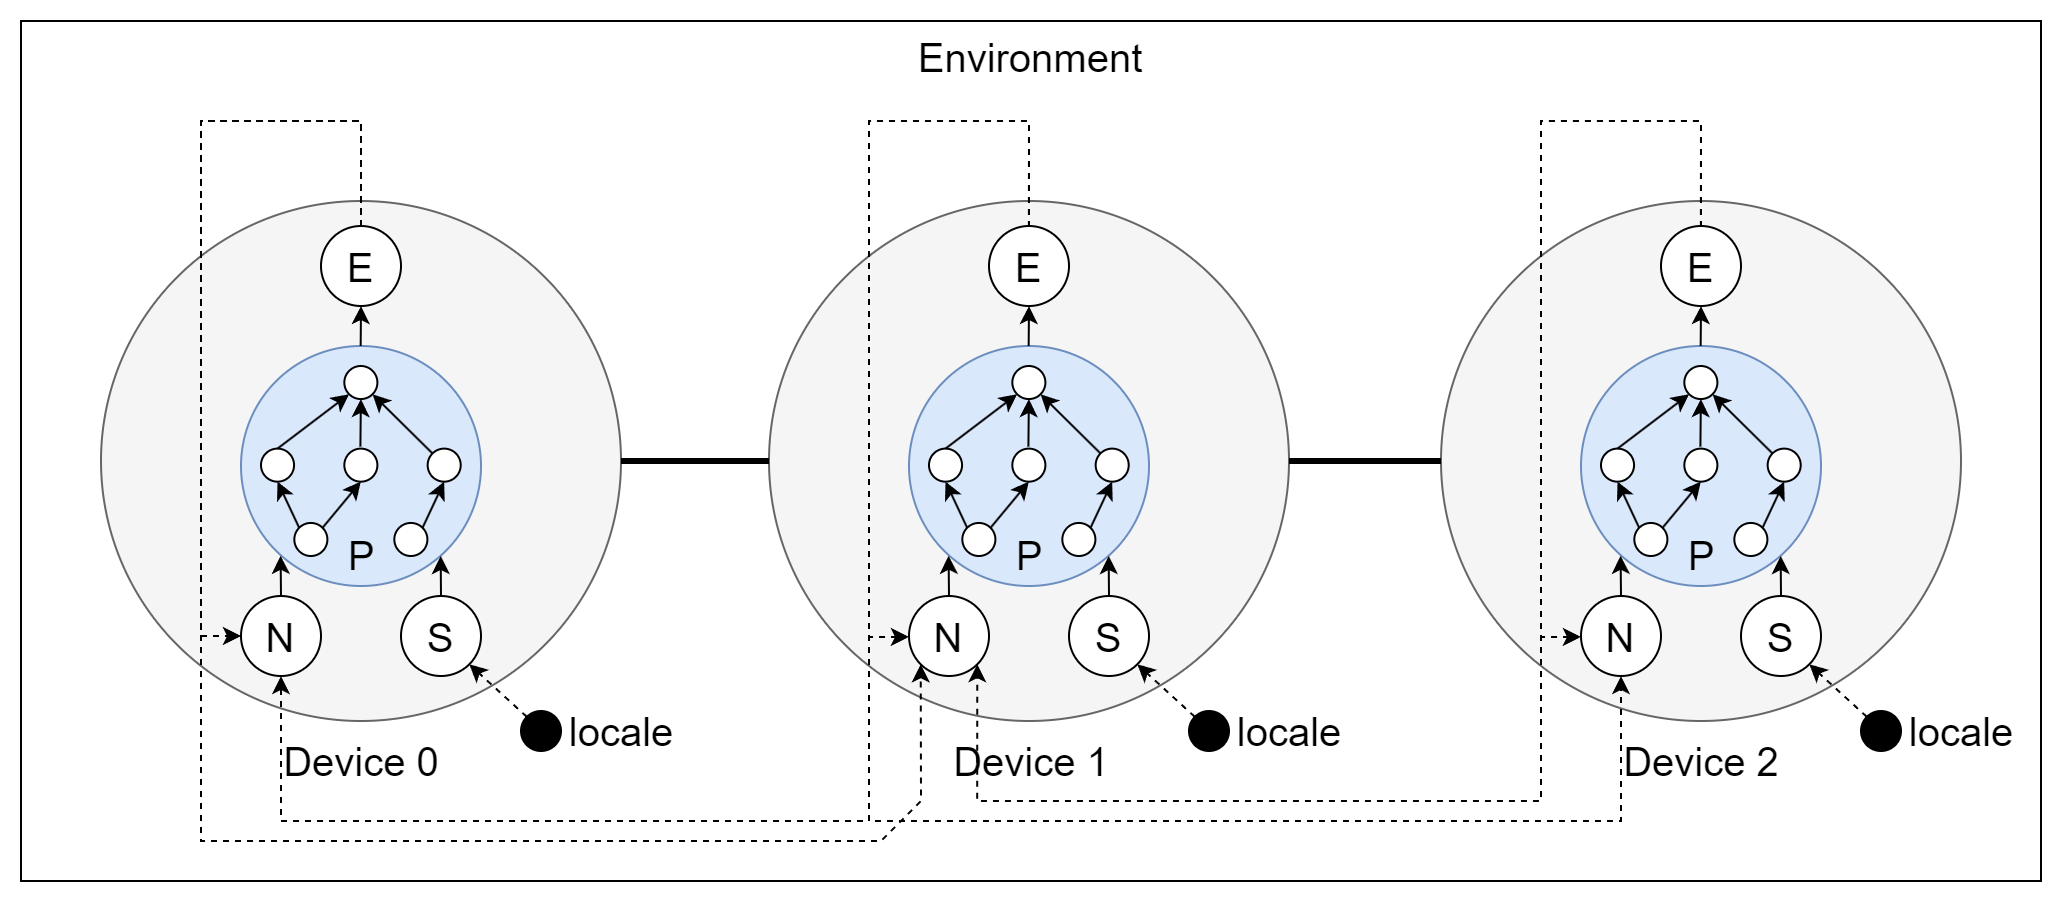
\includegraphics[width=0.89\textwidth]{resources/figures/frasp-simulation.png}
  \caption{
    The reactive execution model of FRASP. In the diagram, three
    devices (\textit{grey circles}) with neighbouring relations (\textit{solid
      lines}) are configured with an aggregate specification (\textit{blue
      circles}). For each device, the input of the specification is
    neighbouring (\textit{nbrs}) and local environmental data (\textit{sense});
    the output is the export trasmitted to neighbours (\textit{export}). In the
    computational graph, there are internal (\textit{solid arrows}) and
    external (\textit{dashed arrows}) dependencies.
  }
  \label{figure:frasp-simulation}
\end{figure}

\begin{figure}[!ht]
  \centering
  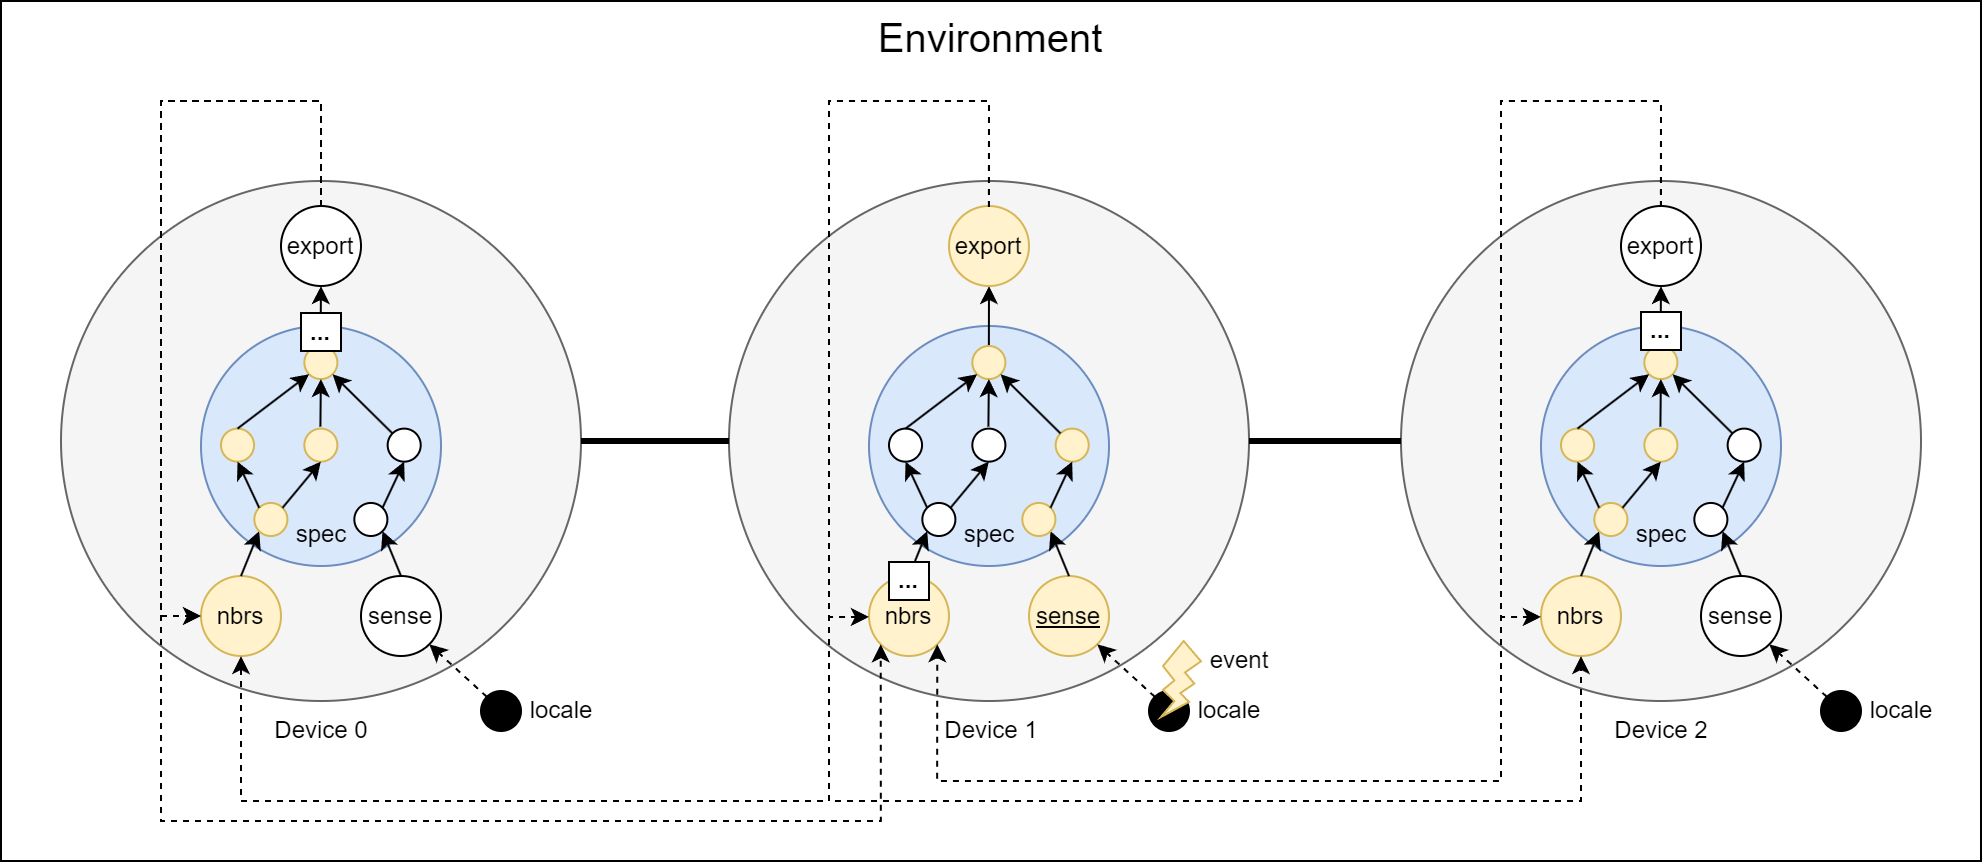
\includegraphics[width=0.89\textwidth]{resources/figures/frasp-simulation-example.png}
  \caption{
    An example of propagation of change in the execution model of FRASP. The
    local environment of device 1 changed, causing changes to all its
    dependents. The three dots indicate that the change continues to
    propagate following the graph dependencies. Note how the
    propagation of change would carry on indefinitely in \textit{any} cyclic
    graph without proper measures (e.g. calming pattern).
  }
  \label{figure:frasp-simulation-example}
\end{figure}

Since this project contributes to the implementation of FRASP, a brief overview
of its architecture is due. Internally, FRASP is organized into the following
three layered modules (Figure \ref{figure:frasp-modules}):
\begin{itemize}
  \item \texttt{frp}: provide extensions and abstractions over the \ac{FRP}
        engine on which the framework depends.
  \item \texttt{core}: provide the model and implementation of the FRASP
        specification, as illustrated previously in Listing
        \ref{listing:frasp-language}.
  \item \texttt{simulation}: provide a basic simulator for running aggregate
        specifications over a network of devices.
\end{itemize}
\begin{figure}[h]
  \centering
  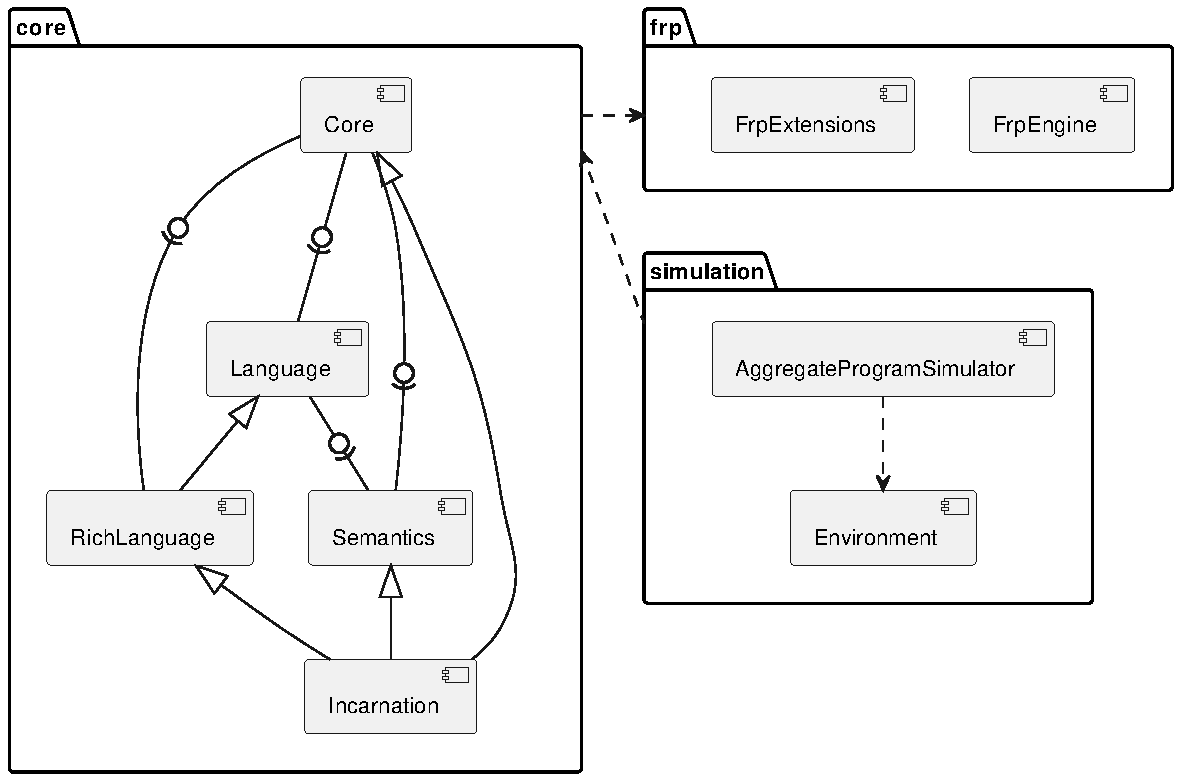
\includegraphics[width=1\textwidth]{resources/figures/frasp-modules.pdf}
  \caption{The architecture of FRASP (image from the paper \cite{FRASP}).}
  \label{figure:frasp-modules}
\end{figure}

The contributions of this project concern mostly the \texttt{frp} and
\texttt{simulation} modules. More details will be provided in the following
chapters as needed.
